  \begin{minipage}[c]{0.4\textwidth}
    \centering
    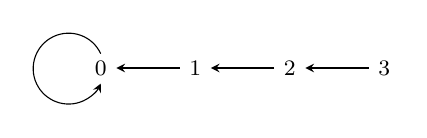
\begin{tikzpicture}[>=stealth, font=\footnotesize,
        node distance=1.2cm and 1.4cm]
      \node (q0) {$0$};
      \node (q1) [right of=q0] {$1$};
      \node (q2) [right of=q1] {$2$};
      \node (q3) [right of=q2] {$3$};
      \draw[->] (q1) -- (q0);
      \draw[->] (q2) to (q1);
      \draw[->] (q3) to (q2);
      \draw[->] ([yshift=5.2pt]q0) arc[start angle=25, end angle=335, radius=4.5mm];
    \end{tikzpicture}
  \end{minipage}%
  \hfill
  \begin{minipage}[c]{0.55\textwidth}
  % >>> print(psi_forest_grid_tikz([8,9,9,9], level=2))
  % and then manually remove \begin{figure} and \end{figure}
  % Kupisch series [8,9,9,9], cokupisch series [8,9,9,9]
\centering
{
\newcommand{\nodea}{\node[draw=none, inner sep=2pt] (a) {}
;}
\newcommand{\nodeb}{\node[draw=none, inner sep=2pt] (b) {}
;}
\newcommand{\nodec}{\node[draw=none, inner sep=2pt] (c) {}
;}
\newcommand{\noded}{\node[draw=none, inner sep=2pt] (d) {}
;}
\newcommand{\nodee}{\node[draw=none, inner sep=2pt] (e) {}
;}
\newcommand{\nodef}{\node[draw=none, inner sep=2pt] (f) {}
;}
\newcommand{\nodeg}{\node[draw=none, inner sep=2pt] (g) {}
;}
\newcommand{\nodeh}{\node[draw=none, inner sep=2pt] (h) {}
;}
\newcommand{\nodei}{\node (i) {$\overline{16}$}
;}
\newcommand{\nodej}{\node (j) {$\overline{15}$}
;}
\newcommand{\nodek}{\node (k) {$\overline{14}$}
;}
\newcommand{\nodel}{\node (l) {$\overline{13}$}
;}
\newcommand{\nodem}{\node (m) {$\overline{12}$}
;}
\newcommand{\noden}{\node (n) {$\overline{11}$}
;}
\newcommand{\nodeo}{\node (o) {$\overline{10}$}
;}
\newcommand{\nodep}{\node (p) {$\overline{9}$}
;}
\newcommand{\nodeq}{\node (q) {$\overline{8}$}
;}
\newcommand{\noder}{\node (r) {$\overline{7}$}
;}
\newcommand{\nodes}{\node (s) {$\overline{6}$}
;}
\newcommand{\nodet}{\node (t) {$\overline{5}$}
;}
\newcommand{\nodeu}{\node (u) {$\overline{4}$}
;}
\newcommand{\nodev}{\node (v) {$\overline{3}$}
;}
\newcommand{\nodew}{\node (w) {$\overline{2}$}
;}
\newcommand{\nodex}{\node (x) {$\overline{1}$}
;}
\newcommand{\nodey}{\node (y) {$0$}
;}
\newcommand{\nodez}{\node (z) {$1$}
;}
\newcommand{\nodeaa}{\node (aa) {$2$}
;}
\newcommand{\nodeab}{\node (ab) {$3$}
;}
\newcommand{\nodeac}{\node (ac) {$4$}
;}
\newcommand{\nodead}{\node (ad) {$5$}
;}
\newcommand{\nodeae}{\node (ae) {$6$}
;}
\newcommand{\nodeaf}{\node (af) {$7$}
;}
\newcommand{\nodeag}{\node (ag) {$8$}
;}
\newcommand{\nodeah}{\node (ah) {$9$}
;}
\newcommand{\nodeai}{\node (ai) {$10$}
;}
\newcommand{\nodeaj}{\node (aj) {$11$}
;}
\newcommand{\nodeak}{\node (ak) {$12$}
;}
\newcommand{\nodeal}{\node (al) {$13$}
;}
\newcommand{\nodeam}{\node (am) {$14$}
;}
\newcommand{\nodean}{\node (an) {$15$}
;}
\newcommand{\nodeao}{\node (ao) {$16$}
;}
\newcommand{\nodeap}{\node (ap) {$17$}
;}
\newcommand{\nodeaq}{\node (aq) {$18$}
;}
\newcommand{\nodear}{\node (ar) {$19$}
;}
\newcommand{\nodeas}{\node (as) {$20$}
;}
\newcommand{\nodeat}{\node (at) {$21$}
;}
\newcommand{\nodeau}{\node (au) {$22$}
;}
\newcommand{\nodeav}{\node (av) {$23$}
;}
\newcommand{\nodeaw}{\node[draw=none, inner sep=2pt] (aw) {}
;}
\newcommand{\nodeax}{\node[draw=none, inner sep=2pt] (ax) {}
;}
\newcommand{\nodeay}{\node[draw=none, inner sep=2pt] (ay) {}
;}
\newcommand{\nodeaz}{\node[draw=none, inner sep=2pt] (az) {}
;}
\newcommand{\nodeba}{\node[draw=none, inner sep=2pt] (ba) {}
;}
\newcommand{\nodebb}{\node[draw=none, inner sep=2pt] (bb) {}
;}
\newcommand{\nodebc}{\node[draw=none, inner sep=2pt] (bc) {}
;}
\newcommand{\nodebd}{\node[draw=none, inner sep=2pt] (bd) {}
;}
\begin{tikzpicture}[auto, font=\footnotesize]
\matrix[column sep=.3cm, row sep=.5cm,ampersand replacement=\&]{
  \nodea  \&  \nodeb  \&  \nodec  \&  \noded  \&  \nodee  \&  \nodef  \&  \nodeg  \&  \nodeh  \\
  \nodei  \&  \nodej  \&  \nodek  \&  \nodel  \&  \nodem  \&  \noden  \&  \nodeo  \&  \nodep  \\
  \nodeq  \&  \noder  \&  \nodes  \&  \nodet  \&  \nodeu  \&  \nodev  \&  \nodew  \&  \nodex  \\
  \nodey  \&  \nodez  \&  \nodeaa  \&  \nodeab  \&  \nodeac  \&  \nodead  \&  \nodeae  \&  \nodeaf  \\
  \nodeag  \&  \nodeah  \&  \nodeai  \&  \nodeaj  \&  \nodeak  \&  \nodeal  \&  \nodeam  \&  \nodean  \\
  \nodeao  \&  \nodeap  \&  \nodeaq  \&  \nodear  \&  \nodeas  \&  \nodeat  \&  \nodeau  \&  \nodeav  \\
  \nodeaw  \&  \nodeax  \&  \nodeay  \&  \nodeaz  \&  \nodeba  \&  \nodebb  \&  \nodebc  \&  \nodebd  \\
};

\path[ultra thick]   (i) edge (q)
	  (i) edge (r)
	  (j) edge (s)
	  (k) edge (t)
	  (m) edge (u)
	  (m) edge (v)
	  (n) edge (w)
	  (o) edge (x)
	  (q) edge (y)
	  (q) edge (z)
	  (r) edge (aa)
	  (s) edge (ab)
	  (u) edge (ac)
	  (u) edge (ad)
	  (v) edge (ae)
	  (w) edge (af)
	  (y) edge (ag)
	  (y) edge (ah)
	  (z) edge (ai)
	  (aa) edge (aj)
	  (ac) edge (ak)
	  (ac) edge (al)
	  (ad) edge (am)
	  (ae) edge (an)
	  (ag) edge (ao)
	  (ag) edge (ap)
	  (ah) edge (aq)
	  (ai) edge (ar)
	  (ak) edge (as)
	  (ak) edge (at)
	  (al) edge (au)
	  (am) edge (av);
\path[ultra thick, dotted]   (a) edge (i)
	  (a) edge (j)
	  (b) edge (k)
	  (c) edge (l)
	  (e) edge (m)
	  (e) edge (n)
	  (f) edge (o)
	  (g) edge (p)
	  (ao) edge (aw)
	  (ao) edge (ax)
	  (ap) edge (ay)
	  (aq) edge (az)
	  (as) edge (ba)
	  (as) edge (bb)
	  (at) edge (bc)
	  (au) edge (bd);
% Colour the three highlighted paths going up through the parents
\path[ultra thick, draw=red]    (i) edge (r)  (r) edge (aa)  (aa) edge (aj);
\path[ultra thick, draw=green]  (m) edge (v)  (v) edge (ae)  (ae) edge (an);
\path[ultra thick, draw=blue]   (i) edge (q)  (q) edge (z)  (z) edge (ai)  (ai) edge (ar);
\begin{pgfonlayer}{background}
% Highlight the start nodes 11, 15, 19 in their path colours
\node[circle, fill=red, opacity=0.35, inner sep=4pt] at (aj) {};
\node[circle, fill=green, opacity=0.35, inner sep=4pt] at (an) {};
\node[circle, fill=blue, opacity=0.35, inner sep=4pt] at (ar) {};
\end{pgfonlayer}
\end{tikzpicture}}
  \end{minipage}%
